\documentclass[12pt, a4paper]{report}

% Packages :

\usepackage[french]{babel}
\usepackage[utf8]{inputenc}
\usepackage[T1]{fontenc}
\usepackage[pdftex, pdfauthor={Bacomathiques}]{hyperref}
\usepackage{sectsty}
\usepackage[explicit]{titlesec}
\usepackage{xcolor}
\usepackage{amsmath}
\usepackage{amssymb}
\usepackage{amsthm}
\usepackage{fourier}
\usepackage{titlesec}
\usepackage{fancyhdr}
\usepackage{catchfilebetweentags}
\usepackage[french, capitalise, noabbrev]{cleveref}
\usepackage[fit, breakall]{truncate}
\usepackage[margin=3cm]{geometry}
\usepackage{tocloft}
\usepackage{tikz}
\usepackage{tocloft}
\usepackage{microtype}
\usepackage{listings}
\usepackage{tabularx}
\usepackage{calc}
\usepackage[export]{adjustbox}
\usepackage[most]{tcolorbox}
\usepackage{standalone}
\usepackage{xlop}
\usepackage{etoolbox}
\usepackage{environ}

\usetikzlibrary{arrows.meta}
\usetikzlibrary{trees}

% Paramètres :

\author{Bacomathiques}
\definecolor{graphe}{HTML}{93c9ff}
\setcounter{MaxMatrixCols}{12}
\setlength{\parindent}{0pt}
\setlength{\fboxsep}{0pt}
%\pdfsuppresswarningpagegroup=1

% Code :

\lstdefinestyle{style}{
	backgroundcolor=\color{white},
	commentstyle=\em\color[HTML]{999988},
	keywordstyle=\bfseries,
	identifierstyle=\normalfont,
	stringstyle=\color[rgb]{0.87, 0.07, 0.27},
	basicstyle=\ttfamily\color{black},
	breakatwhitespace=false,
	breaklines=true,
	captionpos=b,
	keepspaces=true,
	numbers=left,
	numbersep=5pt,
	showspaces=false,
	showstringspaces=false,
	showtabs=false,
	tabsize=2,
	numbers=none
}

\lstset{style=style}
\lstset{
	literate=
	{á}{{\'a}}1
	{à}{{\`a}}1
	{ã}{{\~a}}1
	{é}{{\'e}}1
	{ê}{{\^e}}1
	{í}{{\'i}}1
	{ó}{{\'o}}1
	{õ}{{\~o}}1
	{ú}{{\'u}}1
	{ü}{{\"u}}1
	{ç}{{\c{c}}}1
}

\lstset{
	framextopmargin=10pt,
	framexrightmargin=10pt,
	framexbottommargin=10pt,
	framexleftmargin=10pt,
	xleftmargin=10pt,
	xrightmargin=10pt,
}

% Couleurs :

\definecolor{title}{HTML}{912c21}
\definecolor{section}{HTML}{1c567d}
\definecolor{subsection}{HTML}{2980b9}

\definecolor{rule}{HTML}{c4c4c4}

\definecolor{formula}{HTML}{ebf3fb}
\definecolor{formula-left}{HTML}{3583d6}

\definecolor{tip}{HTML}{dcf3d8}
\definecolor{tip-left}{HTML}{26a65b}

\definecolor{demonstration}{HTML}{fff8de}
\definecolor{demonstration-left}{HTML}{f1c40f}

\definecolor{exercise}{HTML}{e0f2f1}
\definecolor{exercise-left}{HTML}{009688}

\definecolor{correction}{HTML}{e0f7fa}
\definecolor{correction-left}{HTML}{00bcd4}

\definecolor{toc}{HTML}{fceae9}
\definecolor{toc-left}{HTML}{e74c3c}
\definecolor{toc-dark}{HTML}{87281f}

% Titres :

\renewcommand{\thesection}{\Roman{section} - }
\renewcommand{\thesubsection}{\arabic{subsection}. }

\newcommand{\sectionstyle}{\normalfont\LARGE\bfseries\color{section}}
\titleformat{\section}{\sectionstyle}{\thesection #1}{0pt}{}
\titleformat{name=\section, numberless}{\sectionstyle}{#1}{0pt}{}

\newcommand{\subsectionstyle}{\normalfont\Large\bfseries\color{subsection}}
\titleformat{\subsection}{\subsectionstyle}{\thesubsection #1}{0pt}{}
\titleformat{name=\subsection, numberless}{\subsectionstyle}{#1}{0pt}{}

\titlelabel{\thetitle\ }

% Table des matières :

\addto\captionsfrench{\renewcommand\contentsname{}}
\renewcommand{\cftsecpagefont}{\color{toc-dark}}
\renewcommand{\cftsubsecpagefont}{\color{toc-dark}}
\renewcommand{\cftsecleader}{\cftdotfill{\cftdotsep}}
\renewcommand{\cftsecfont}{\bfseries}
\renewcommand{\cftsecpagefont}{\bfseries\color{toc-dark}}
\setlength{\cftbeforetoctitleskip}{0pt}
\setlength{\cftaftertoctitleskip}{0pt}
\setlength{\cftsecindent}{0pt}
\setlength{\cftsubsecindent}{20pt}
\setlength{\cftsubsecnumwidth}{20pt}

% Commandes :

\newcommand{\newpar}{\\[\medskipamount]}
\newcommand{\lesson}[3]{%
	\newcommand{\level}{#1}%
	\newcommand{\id}{#2}%
	\hypersetup{pdftitle={#3}}
	\begin{center}%
		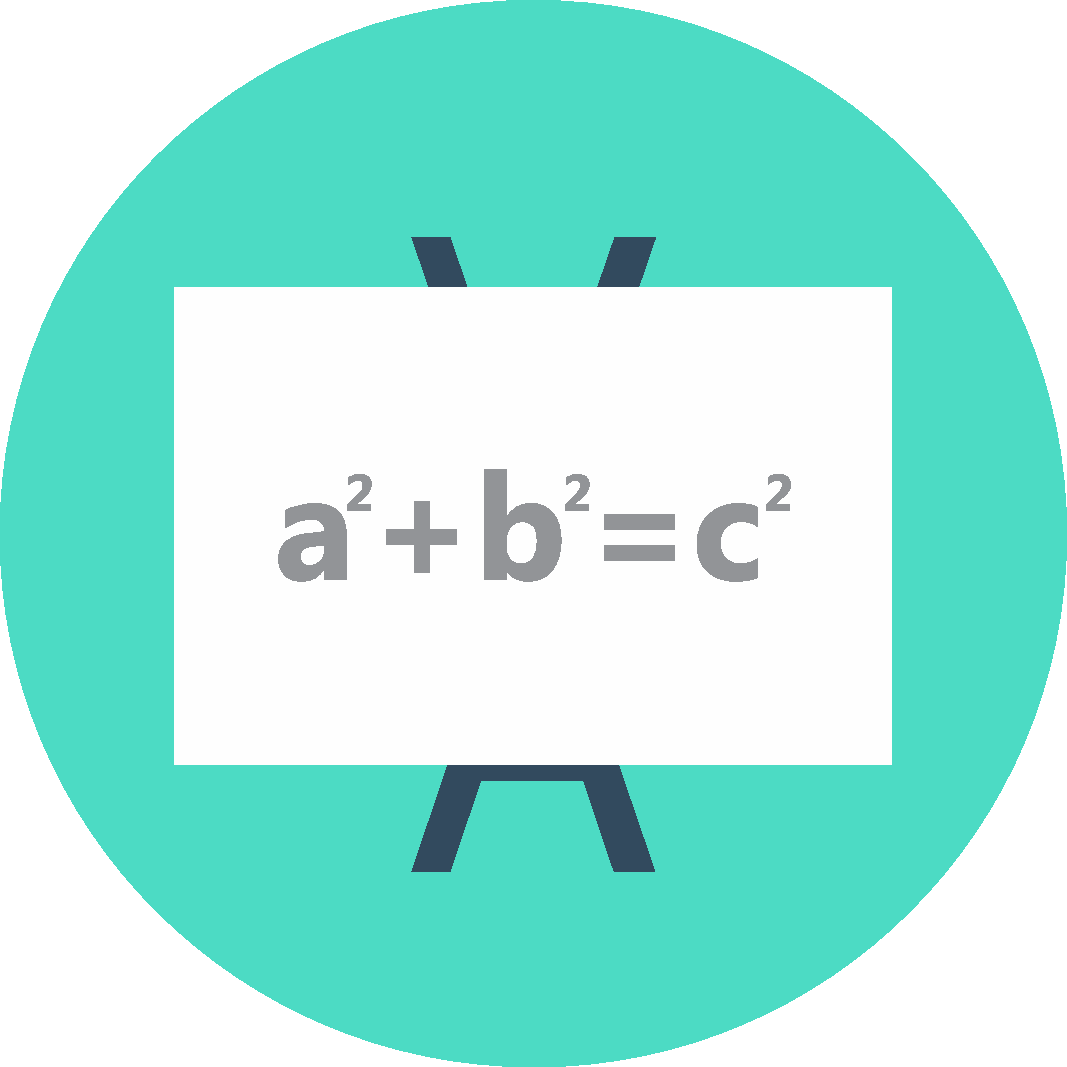
\includegraphics[width=150px]{\imagespath/bacomathiques}%
		
		\vspace{30pt}%
		{\Huge\color{title} #3}%
		
		\vspace{10pt}%
		{Bacomathiques --- \href{https://bacomathiqu.es/cours/#1/#2}{\color{section} https://bacomathiqu.es}}%
		
		\vspace{20pt}%
	\end{center}%
	\begin{toc}
		\tableofcontents%
	\end{toc}
	\thispagestyle{empty}%
	\newpage%
	\setcounter{page}{1}%
}
\newcommand{\imagespath}{../../images}
\newcommand{\lessonimagespath}{\imagespath/lessons/\level/\id/}
\newcommand{\includelatexpicture}[2][\textwidth - 100pt]{%
	\begin{center}%
		\resizebox{#1}{!}{%
			\input{\lessonimagespath#2}%
		}%
	\end{center}%
	\medskip%
}
\newcommand{\includeimage}[1]{%
	\begin{center}%
		\includegraphics{\lessonimagespath#1}%
	\end{center}%
	\medskip%
}
\newcommand{\includerepresentation}[1]{%
	\begin{center}%
		\setlength{\fboxrule}{0.5pt}%
		\href{https://www.geogebra.org/m/#1}{\includegraphics[width=\textwidth-1pt,fbox]{\lessonimagespath#1}}%
	\end{center}%
}
\newcommand{\floor}[1]{\lfloor #1 \rfloor}

\makeatletter
\newcommand\inputcontent{\@ifstar{\inputcontent@star}{\inputcontent@nostar}}
\newcommand{\inputcontent@star}[1]{%
	\ExecuteMetaData[#1]{content}%
}
\newcommand{\inputcontent@nostar}[1]{%
	\newpage%
	\inputcontent@star{#1}%
}
\makeatother

\let\oldsection\section
\renewcommand\section{\clearpage\oldsection}
\newcommand{\contentwidth}[1][medium]{}

% En-têtes :

\pagestyle{fancy}

\renewcommand{\sectionmark}[1]{\markboth{\thesection \ #1}{}}

\fancyhead[R]{\truncate{0.23\textwidth}{\color{title}\thepage}}
\fancyhead[L]{\truncate{0.73\textwidth}{\color{title}\leftmark}}
\fancyfoot[C]{\scriptsize \href{https://bacomathiqu.es/cours/\level/\id}{\texttt{bacomathiqu.es}}}

\makeatletter
\patchcmd{\f@nch@head}{\rlap}{\color{rule}\rlap}{}{}
\patchcmd{\headrule}{\hrule}{\color{rule}\hrule}{}{}
\makeatother

% Environnements :

\newenvironment{nosummary}{}{}
\newcommand{\tcolorboxtitle}[2]{\setlength{\fboxsep}{2.5pt}\hspace{-10pt}\colorbox{#1-left}{\hspace{8pt}\MakeUppercase{#2} \hspace{2pt} \includegraphics[height=0.8em]{\imagespath/bubbles/#1}\hspace{5pt}}}
\newcommand{\tcolorboxsubtitle}[2]{\ifstrempty{#2}{}{\textcolor{#1-left}{\large#2}\\[\medskipamount]}}
\tcbset{
	frame hidden,
	boxrule=0pt,
	boxsep=0pt,
	enlarge bottom by=8.5pt,
	enhanced jigsaw,
	boxed title style={sharp corners,boxrule=0pt,coltitle={white},titlerule=0pt},
	fonttitle=\fontsize{6pt}{6pt}\bfseries\boldmath,
	top=10pt,
	right=10pt,
	bottom=10pt,
	left=10pt,
	arc=0pt,
	outer arc=0pt,
}
\newtcolorbox{toc}[1][]{
	colback=toc,
	borderline west={3pt}{0pt}{toc-left},
	title=\tcolorboxtitle{toc}{Table des matières},
	colbacktitle=toc,
	before upper={\tcolorboxsubtitle{toc}{#1}}
}
\newtcolorbox{formula}[1][]{
	colback=formula,
	borderline west={3pt}{0pt}{formula-left},
	title=\tcolorboxtitle{formula}{À retenir},
	colbacktitle=formula,
	before upper={\tcolorboxsubtitle{formula}{#1}}
}
\newtcolorbox{tip}[1][]{
	colback=tip,
	borderline west={3pt}{0pt}{tip-left},
	title=\tcolorboxtitle{tip}{À lire},
	colbacktitle=tip,
	before upper={\tcolorboxsubtitle{tip}{#1}}
}
\newtcolorbox{demonstration}[1][]{
	colback=demonstration,
	borderline west={3pt}{0pt}{demonstration-left},
	title=\tcolorboxtitle{demonstration}{Démonstration},
	colbacktitle=demonstration,
	before upper={\tcolorboxsubtitle{demonstration}{#1}}
}

\NewEnviron{whitetabularx}[1]{%
	\renewcommand{\arraystretch}{2.5}
	\colorbox{white}{%
		\begin{tabularx}{\textwidth}{#1}%
			\BODY%
		\end{tabularx}%
	}%
}

% Longueurs :

\newlength{\espacetitreliste}
\setlength{\espacetitreliste}{-16pt}
\newcommand{\entretitreetliste}{\vspace{\espacetitreliste}}

\begin{document}
	%<*content>
	\lesson{terminale}{arithmetique}{Chapitre XIV -- Arithmétique (Maths expertes)}
	
	\section{Divisibilité et congruence}
	
	\subsection{Divisibilité}
	
	Dans toute la suite de cette section, on notera par $\mathbb{Z}$ l'ensemble des nombres entiers relatifs (i.e. $\mathbb{Z} = \{\dots, -2, -1, 0, 1, 2, \dots\}$) et par $\mathbb{N}$ l'ensemble des nombres entiers naturels (i.e. $\mathbb{N} = \{0, 1, 2, \dots\}$).
	
	\begin{formula}[Définition]
		Soient $a$ et $b$ deux entiers relatifs. On dit que $b$ \textbf{divise} $a$ (ou que $a$ est \textbf{un multiple} de $b$) s'il existe $k \in \mathbb{Z}$ tel que $a = kb$. On note ceci par $b \mid a$.
	\end{formula}
	
	\begin{tip}
		Si on a $b$ divise $a$, alors $-b$ divise $a$. Par exemple, comme $6$ divise $12$, alors $-6$ divise également $12$.
	\end{tip}
	
	\begin{formula}[Propriétés]
		\entretitreetliste
		\begin{itemize}
			\item Tout entier relatif $b$ divise $0$ (car $0 = 0 \times b$).
			\item $1$ divise tout entier relatif $a$ (car $a = a \times 1$).
			\item Si $c \mid a$ et $c \mid b$ alors $c \mid (au + bv)$ pour tout $u$, $v \in \mathbb{Z}$.
		\end{itemize}
	\end{formula}
	
	\subsection{Division euclidienne}
	
	La \textbf{division euclidienne} est une notion mathématique que l'on aborde très tôt au cours de notre scolarité (dès la classe de CM1). Nous allons tenter de formaliser ceci :
	
	\begin{formula}[Théorème de la division euclidienne]
		Soient $a$, $b \in \mathbb{Z}$. On suppose $b \neq 0$. On appelle \textbf{division euclidienne} de $a$ par $b$, l'opération qui à $(a, b)$, associe le couple d'entiers relatifs $(q, r)$ tel que $a = bq + r$ où $0 \leq r < |b|$. Un tel couple \textbf{existe} forcément et est \textbf{unique}.
	\end{formula}
	
	\begin{formula}[Vocabulaire]
		En reprenant les notations du théorème, $a$ s'appelle le \textbf{dividende}, $b$ le \textbf{diviseur}, $q$ le \textbf{quotient} et $r$ le \textbf{reste} de la division euclidienne.
	\end{formula}
	
	\begin{tip}[Exemple]
		On souhaite effectuer la division euclidienne de $314$ par $7$. Posons-la :
		\includelatexpicture[100pt]{division-euclidienne}
		\begin{itemize}
			\item On cherche combien de fois $7$ est contenu dans $31$ (cela ne sert à rien de commencer par $3$ car $3 < 7$). On a $4 \times 7 = 28$ et $5 \times 7 = 35$ donc on écrit $4$ sous le diviseur et le reste $31 - 28 = 3$. Puis, on abaisse le chiffre des unités qui est $4$.
			\item On recommence : combien de fois $7$ est-il contenu dans $34$ ? Comme $4 \times 7 = 28$ et $5 \times 7 = 35$, $7$ est contenu $4$ fois dans $34$ et il reste $34 - 28 = 6$.
			\item Comme $6 < 7$, la division euclidienne est terminée : on a $314 = 7 \times 44 + 6$.
		\end{itemize}
	\end{tip}
	
	Donnons enfin une propriété qui nous sera utile dans la section suivante.
	
	\begin{formula}[Propriété]
		Soit $n \in \mathbb{N}$ tel que $n \neq 0$. Deux entiers relatifs $a$ et $b$ ont le même reste dans la division euclidienne par $n$ si et seulement si $a-b$ est un multiple de $n$.
	\end{formula}
	
	\subsection{Congruences dans $\mathbb{Z}$}
	
	\begin{formula}[Définition]
		On dit que deux entiers relatifs $a$ et $b$ sont \textbf{congrus modulo $n$} (où $n$ est un entier naturel supérieur ou égal à $2$) si $a$ et $b$ ont le même reste dans la division euclidienne par $n$. On note alors $a \equiv b \mod n$.
	\end{formula}
	
	\begin{tip}
		On remarque que $a$ est un multiple de $n$ si et seulement si $a \equiv 0 \mod n$.
	\end{tip}
	
	\begin{tip}[Exemple]
		Par exemple, $1 \equiv 4 \equiv 7 \mod 3$.
		\includelatexpicture{congruences}
	\end{tip}
	
	On signale que la congruence est une \textbf{relation d'équivalence}.
	
	\begin{formula}[Propriétés]
		Soit $n \geq 2$. Pour tout $a$, $b$, $c \in \mathbb{Z}$ :
		\begin{itemize}
			\item $a \equiv a \mod n$ (\textbf{réflexivité})
			\item Si $a \equiv b \mod n$, alors $b \equiv a \mod n$ (\textbf{symétrie})
			\item Si $a \equiv b \mod n$, et si $b \equiv c \mod n$, alors $a \equiv c \mod n$ (\textbf{transitivité})
		\end{itemize}
	\end{formula}
	
	De plus, la congruence est compatible avec les opérations usuelles sur les entiers relatifs.
	
	\begin{formula}[Propriétés]
		Soit $n \geq 2$. Soient $a$, $b$, $c$ et $d \in \mathbb{Z}$ tels que $a \equiv b \mod n$ et $c \equiv d \mod n$. Alors on a la compatibilité avec :
		\begin{itemize}
			\item L'\textbf{addition} : $a + c \equiv b + d \mod n$.
			\item La \textbf{multiplication} : $ac \equiv bd \mod n$.
			\item Les \textbf{puissances} : pour tout $k \in \mathbb{N}$, $a^k \equiv b^k \mod n$.
		\end{itemize}
	\end{formula}
	
	\begin{tip}[Exemple]
		Comme $7 \equiv 3 \mod 4$, et $5 \equiv 1 \mod 4$, on a $35 = 5 \times 7 \equiv 1 \times 5 \mod 4$.
	\end{tip}
	
	\section{PGCD et théorème de Bézout}
	
	\subsection{Plus Grand Commun Diviseur}
	
	\begin{formula}[Définition]
		Soient $a$, $b \in \mathbb{Z}$ non tous nuls. Le \textbf{Plus Grand Commun Diviseur} de $a$ et $b$ (noté $\operatorname{PGCD}(a; b)$) est le plus grand entier positif qui les divise simultanément.
	\end{formula}
	
	Avec cette définition, on peut dégager quelques propriétés.
	
	\begin{formula}[Propriétés]
		Soient $a$, $b \in \mathbb{Z}$ non tous nuls.
		\begin{itemize}
			\item $\operatorname{PGCD}(a; b) = \operatorname{PGCD}(b; a)$
			\item $\operatorname{PGCD}(a; 1) = 1$
			\item $\operatorname{PGCD}(a; 0) = a$
			\item Pour tout $k \in \mathbb{N}$, $\operatorname{PGCD}(ka; kb) = k \operatorname{PGCD}(a; b)$
			\item Si $b \mid a$, alors $\operatorname{PGCD}(a; b) = |b|$
		\end{itemize}
	\end{formula}
	
	Il existe une manière de déterminer le $\operatorname{PGCD}$ de deux entiers naturels non nuls $a$ et $b$ avec $b < a$ appelée \textbf{Algorithme d'Euclide}.
	
	\begin{formula}[Algorithme d'Euclide]
		Soient $a$, $b \in \mathbb{Z}$ non tous nuls. Pour obtenir $\operatorname{PGCD}(a; b)$, on procède comme suit :
		\begin{enumerate}
			\item On fait la division euclidienne de $a$ par $b$ et on appelle $r$ le reste.
			\item Si $r = 0$, alors $\operatorname{PGCD}(a; b) = b$.
			\item Sinon on recommence l'étape 1 en remplaçant $a$ par $b$ et $b$ par $r$.
		\end{enumerate}
	\end{formula}
	
	Terminons cette section par une définition.
	
	\begin{formula}[Nombres premiers entre eux]
		On dit que deux nombres sont \textbf{premiers entre eux} si leur $\operatorname{PGCD}$ est égal à 1.
	\end{formula}
	
	\begin{tip}
		Petite remarque : si on note $d$ le $\operatorname{PGCD}$ de deux nombres $a$ et $b$, alors $\frac{a}{d}$ et $\frac{b}{d}$ sont deux nombres premiers entre eux.
	\end{tip}
	
	\subsection{Théorème de Bézout}
	
	Un résultat fondamental de l'arithmétique est le \textbf{théorème de Bachet-Bézout} (que l'on rencontre parfois sous le nom d'\textbf{identité de Bézout}).
	
	\begin{formula}[Théorème de Bachet-Bézout]
		Soient $a$ et $b$ deux entiers relatifs non nuls. On note $d$ leur PGCD. Alors il existe deux entiers relatifs $u$ et $v$ tels que $ua + vb = d$.
	\end{formula}
	
	\begin{formula}[Théorème de Bézout]
		Une conséquence de ce théorème est que $a$ et $b$ sont premiers entre eux si et seulement s'il existe deux entiers relatifs $u$ et $v$ tels que $ua + vb = 1$.
	\end{formula}
	
	\begin{tip}[Exemple]
		Calculons $\operatorname{PGCD}(250; 150)$ et déduisons-en deux entiers relatifs $u$ et $v$ tels que $50 = 250u + 150v$.
		Commençons par calculer le $\operatorname{PGCD}$ de $250$ et $150$ par l'algorithme d'Euclide :
		\newpar
		La division euclidienne de $250$ par $150$ donne $250 = 150 \times 1 + 100$.
		\newline
		La division euclidienne de $150$ par $100$ donne $150 = 100 \times 1 + 50$.
		\newline
		La division euclidienne de $100$ par $50$ donne $100 = 5 \times 2 + 0$.
		\newpar
		On a $\operatorname{PGCD}(250;150) = 50$. Déterminons $u$ et $v$ :
		\newpar
		$250 = 150 \times 1 + 100 \iff 150 = 1 \times 250 - 1 \times 100$
		\newline
		$150 = 1 \times 100 + 50 \iff 50 = 150 - 1 \times 100$
		\newpar
		Donc $50 = 1 \times 250 - 1 \times 100 - 1 \times 100 = 1 \times 250 - 2 \times 100$.
		\newpar
		On a par conséquent $u = 1$ et $v = -2$. L'algorithme que l'on vient d'utiliser pour trouver $u$ et $v$ s'appelle l'\textbf{algorithme d'Euclide étendu}.
	\end{tip}
	
	\begin{formula}[Résolution d'une congruence simple]
		Supposons que l'on souhaite résoudre une congruence du type $ax \equiv b \mod n$ d'inconnue $x$. On pose $d = \operatorname{PGCD(a; n)}$. Alors :
		\begin{enumerate}
			\item Si $d$ ne divise pas $b$, on cherche deux entiers $u$ et $v$ tels que $au + nv = 1$ (avec l'algorithme d'Euclide étendu par exemple). Les solutions de la congruence sont alors les entiers $x$ vérifiant $x \equiv ub \mod n$.
			\item Si $d \mid b$, cela revient à résoudre la congruence $\frac{a}{d}x \equiv \frac{b}{d} \mod \frac{n}{d}$, et on se ramène au cas 1 (avec la nouvelle congruence à résoudre).
		\end{enumerate}
	\end{formula}
	
	\begin{tip}[Exemple]
		On souhaite résoudre la congruence $6x \equiv 6 \mod 9$. Alors, comme $d = \operatorname{PGCD}(6; 9) = 3$, on a $d \mid 6$. On se ramène donc à résoudre $2x \equiv 2 \mod 3$ (où $2$ et $3$ sont premiers entre eux).
		\newpar
		On écrit l'identité de Bézout appliquée à $2$ et $3$ : $2 \times 2 + 3 \times -1 = 1$. Donc les solutions à la congruence du début sont les entiers $x$ vérifiant $x \equiv 4 \mod 3 \equiv 1 \mod 3$ (i.e. les $x$ de la forme $x = 3k + 1$ où $k \in \mathbb{Z}$).
	\end{tip}
	
	\subsection{Lemme de Gauss}
	
	\begin{formula}[Lemme de Gauss]
		Soient $a$, $b$ et $c$ trois entiers non nuls. Si $c \mid ab$ et $c$ est premier avec $a$, alors $c \mid b$.
	\end{formula}
	
	\begin{formula}[Corollaire]
		Soient $a$, $b$ et $c$ trois entiers non nuls. Si $b \mid a$, $c \mid a$ et que $b$ et $c$ sont premiers entre eux, alors $bc \mid a$.
	\end{formula}
	
	\subsection{Équations diophantiennes}
	
	\begin{formula}[Définition]
		Une \textbf{équation diophantienne linéaire en deux variables} $x$ et $y$ est une équation de la forme $(E) : ax + by = c$ où les coefficients $a$, $b$ et $c$ sont des entiers relatifs et où les solutions sont également des entiers relatifs.
	\end{formula}
	
	\begin{formula}[Solutions de $(E)$]
		En reprenant les notations précédentes, on pose $d = \operatorname{PGCD}(a; b)$. Alors :
		\begin{itemize}
			\item Si $d \mid c$, on cherche une solution particulière à $(E)$ que l'on note $(x_0; y_0)$. Alors les solutions de $(E)$ sont les couples $(x_k; y_k)$ où $x_k = x_0 + k\frac{b}{d}$ et $y_k = y_0 - k\frac{a}{d}$.
			\item Sinon, $(E)$ n'a pas de solution.
		\end{itemize}
	\end{formula}
	
	\begin{tip}[Exemple]
		On cherche à résoudre l'équation diophantienne $(E) : 25x + 10y = 15$. Commençons par chercher une solution particulière $(x_0; y_0)$.
		\newpar
		Comme $d = \operatorname{PGCD}(25; 10) = 5$, on a $d \mid 15$. En divisant les deux côtés de l'égalité par $5$, on a $(E) \iff 5x + 2y = 3$.
		\newpar
		Cherchons une solution particulière à $(E)$. On écrit l'identité de Bézout appliquée à $5$ et $2$ : $5 \times 1 + 2 \times -2 = 1$. Ainsi, en multipliant les deux côtés de l'égalité par $3$, on obtient : $5 \times 3 + 2 \times -6 = 3$.
		\newpar
		On a trouvé une solution particulière à $(E)$ qui est le couple $(x_0; y_0$) où $x_0 = 3$ et $y_0 = -6$. On pourrait appliquer la formule pour donner la forme générale des solutions de $(E)$, mais essayons de ne pas l'utiliser.
		\newpar
		Soit $(x; y)$ une autre solution de $(E)$. On a $3 = 5x + 2y = 5x_0 + 2y_0$. D'où $5(x - x_0) = 2(y_0 - y)$ (en passant les $x$ et $x_0$ du même côté de l'égalité et en faisant de même pour $y$ et $y_0$, puis en factorisant).
		\newpar
		Ainsi, on a $5 \mid 2(y_0 - y)$. Or, $5$ et $2$ sont premiers entre eux, donc par le lemme de Gauss, $5 \mid y_0 - y$. Il existe donc $q_1$ tel que $5q_1 = y_0 - y$, d'où $y = y_0 - 5q_1$.
		\newpar
		De même, $2 \mid 5(x - x_0)$ avec $2$ et $5$ premiers entre eux, donc par le lemme de Gauss, $2 \mid x - x_0$. Il existe donc $q_2$ tel que $2q_2 = x - x_0$, d'où $x = x_0 + 2q_2$.
		\newpar
		En réinjectant tout ça dans $(E)$, on obtient $5(x_0 + 2q_2) + 2(y_0 + -5q_1) = 3 \iff \underbrace{5x_0 + 2y_0}_{= 3} + 10q_2 - 10q_1 = 3 \iff q_1 = q_2$.
		\newpar
		Les solutions de $(E)$ sont donc les couples $(x_k; y_k)$ où $x_k = x_0 + 2k$ et $y_k = y_0 - 5k$ (et on a bien les mêmes résultats qu'avec la formule).
	\end{tip}
	
	\section{Nombres premiers}
	
	\subsection{Définition}
	
	Commençons cette section par définir ce qu'est un \textbf{nombre premier}. Il s'agit là d'une notion dont entend parler très tôt au cours de notre scolarité, sans pour autant vraiment rentrer dans le sujet. Détaillons donc un peu tout ceci.
	
	\begin{formula}[Nombre premier]
		Un nombre entier $p \geq 2$ est dit \textbf{premier} si ses seuls diviseurs positifs sont $1$ et lui-même.
	\end{formula}
	
	\begin{tip}[Exemple]
		$2$, $3$, $5$, $7$, $11$ et $13$ sont des nombres premiers.
	\end{tip}
	
	\subsection{Propriétés}
	
	Voici quelques propriétés basiques que possèdent les nombres premiers.
	
	\begin{formula}[Propriétés]
		Soit $n \in \mathbb{N}$ supérieur ou égal à 2, alors on a les propriétés suivantes :
		\begin{itemize}
			\item Si $n$ n'admet aucun diviseur premier inférieur ou égal à $\sqrt{n}$, alors $n$ est premier.
			\item Si $n$ n'est pas premier alors $n$ admet au moins un diviseur premier inférieur ou égal à $\sqrt{n}$.
			\item Si $n$ est premier et $n$ ne divise pas un entier $m$, alors $n$ et $m$ sont premiers entre eux.
		\end{itemize}
	\end{formula}
	
	\begin{formula}[Lemme d'Euclide]
		Soit $p$ un nombre premier et $a$ et $b$ deux entiers. Si $p \mid ab$ alors $p \mid a$ ou $p \mid b$.
	\end{formula}
	
	On donne enfin un résultat fondamental (mais qui reste très simple) sur l'ensemble des nombres premiers.
	
	\begin{formula}[Infinité de nombres premiers]
		Il existe une infinité de nombres premiers.
	\end{formula}
	
	\begin{demonstration}[Infinité de nombres premiers]
		Supposons par l'absurde que l'ensemble des nombres premiers soit un ensemble fini. On note par $P$ cet ensemble et par $r$ sont cardinal. On a donc $P = \{p_1, p_2, \dots, p_r\}$ où $p_1$, $p_2$, ... , $p_r$ sont premiers. \newpar
		Soit $N = p_1 \times p_2 \times \dots \times p_r + 1$. Alors, $N \notin P$ donc $N$ n'est pas premier (et est strictement supérieur à $1$). Il existe donc un nombre premier qui divise $N$.
		\newpar
		En d'autres mots, il existe $i \in \{1, \dots, r\}$ tel que $p_i \mid N$. De plus, $p_i \mid p_1 \times p_2 \times \dots \times p_r$.
		\newpar
		Donc $p_i \mid N -  p_1 \times p_2 \times \dots \times p_r \iff p_i \mid 1$, donc $p_i = 1$ ou $p_i = 0$ : c'est absurde car $p_i \geq 2$.
		\newpar
		Pour la petite histoire, c'est Euclide qui a fourni une première version de cette preuve en 300 av. J.-C !
	\end{demonstration}
	
	\begin{formula}[Petit théorème de Fermat]
		\label{thm:fermat}
		Soit $p$ un nombre premier et $a$ un entier non divisible par $p$. Alors $a^{p-1} \equiv 1 \mod p$.
	\end{formula}
	
	\begin{tip}
		Cela revient au même de dire que si $a$ est un entier quelconque et que $p$ est un nombre premier, alors $a^p \equiv a \mod p$.
	\end{tip}
	
	\subsection{Décomposition de nombres}
	
	Passons maintenant à un résultat fondamental de l'arithmétique : le principe de \textbf{décomposition en produit de facteurs premiers} (il s'agit même là d'un théorème qui est sobrement intitulé \textbf{théorème fondamental de l'arithmétique}).
	
	\begin{formula}[Théorème fondamental de l'arithmétique]
		Soit $n \in \mathbb{N}$ supérieur ou égal à 2, alors $n$ peut s'écrire de la façon suivante :
		\[ n = p_{1}^{\alpha_1} \times p_{2}^{\alpha_2} \times \dots \times p_{n}^{\alpha_n} \]
		où $p_1$, $p_2$, ... , $p_n$ des nombres premiers tels que $p_1 < p_2 < \dots < p_n$ et $\alpha_1$, $\alpha_2$, ... , $\alpha_n$ des entiers naturels non nuls.
	\end{formula}
	
	\begin{tip}[Exemple]
		Décomposons $200$ en produit de facteurs premiers.
		\begin{itemize}
			\item $200 = 2 \times 100$ ($2$ est le plus petit nombre premier qui divise $200$).
			\item $100 = 2 \times 50$ ($2$ est le plus petit nombre premier qui divise $100$).
			\item $50 = 2 \times 25$ ($2$ est le plus petit nombre premier qui divise $50$).
			\item $25 = 5 \times 5$ ($5$ est le plus petit nombre premier qui divise $25$).
			\item $5 = 5 \times 1$ ($5$ est un nombre premier, c'est terminé).
		\end{itemize}
		On a donc $200 = 2 \times 100 = 2 \times (2 \times 50) = \dots = 2^3 \times 5^2$.
	\end{tip}
	%</content>
\end{document}